\documentclass[a4paper,10pt]{article}
\usepackage[utf8]{inputenc}
\usepackage[spanish]{babel}
\usepackage[affil-it]{authblk}
\usepackage{enumerate}
\usepackage{graphicx}
\usepackage{hyperref}
\usepackage{amsmath}
\usepackage{amssymb}
\usepackage{cancel}
\usepackage{tikz}
\usepackage{float}
\usepackage{cleveref}
\usepackage[margin=1.4in]{geometry}
\usepackage[labelfont=bf]{caption}
\usetikzlibrary{calc}
\numberwithin{equation}{section}

%Indentation
\setlength{\parindent}{0ex}

%Multiple References

\usepackage{xparse}
\ExplSyntaxOn
\NewDocumentCommand{\mref}{m}{\quinn_mref:n {#1}}
\seq_new:N \l_quinn_mref_seq
\cs_new:Npn \quinn_mref:n #1
 {
  \seq_set_split:Nnn \l_quinn_mref_seq { , } { #1 }
  \seq_pop_right:NN \l_quinn_mref_seq \l_tmpa_tl
  ( % print the left parenthesis
  \seq_map_inline:Nn \l_quinn_mref_seq
    { \ref{##1},\nobreakspace } % print the first references
  \exp_args:NV \ref \l_tmpa_tl 
  ) 
 }
\ExplSyntaxOff


%Boxes

\newcommand*{\boxcolor}{blue}
\makeatletter
\renewcommand{\boxed}[1]{\textcolor{\boxcolor}{%
\tikz[baseline={([yshift=-1ex]current bounding box.center)}] \node [rectangle, minimum width=1ex,rounded corners,draw] {\normalcolor\m@th$\displaystyle#1$};}}
 \makeatother

%Constantes
\newcommand{\euler}{\mathrm{e}}
\newcommand{\im}{i}

%Lemas, teoremas, definiciones y pruebas
\newcommand{\definicion}{\textbf{Definición: }}
\newcommand{\lema}{\textbf{Lema: }}
\newcommand{\teorema}{\textbf{Teorema: }}
\newcommand{\prueba}{\textbf{Prueba: }}


%opening
\title{Mecánica Clásica Tarea \# 3}
\author{Favio Vázquez\thanks{Correo: favio.vazquezp@gmail.com}}\affil{Instituto de Ciencias Nucleares. Universidad Nacional Autónoma de México.}
\date{}

\begin{document}

\makeatletter
\def\@maketitle{%
  \newpage
  \null
  \vskip 2em%
  \begin{center}%
  \let \footnote \thanks
    {\Large\bfseries \@title \par}%
    \vskip 1.5em%
    {\normalsize
      \lineskip .5em%
      \begin{tabular}[t]{c}%
        \@author
      \end{tabular}\par}%
    \vskip 1em%
    {\normalsize \@date}%
  \end{center}%
  \par
  \vskip 1.5em}
\makeatother

\maketitle

\section{Problema 1}

Trace el diagrama o retrato de fase que corresponde al movimiento de una
partícula en una dimensión sujeta al potencial que se ilustra en la 
figura.

\begin{figure}[H]
 \center 
 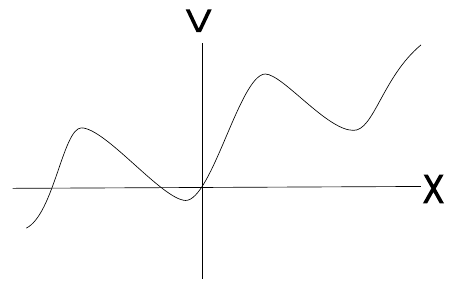
\includegraphics[scale=0.5]{problema1fig1}
 \caption{Problema 1. Diagrama del potencial a estudiar}
\end{figure}

\vspace{.3cm}

\underline{Solución:} \vspace{.3cm}

En el gráfico del potencial a estudiar es fácil notar que, en la porción dada, hay 
dos mínimos y dos máximos (casi se puede ver el tercero) pronunciados, en los mínimos tendremos en el retrato 
de fases centros y en los máximos puntos de silla. El retrato de fase resultante es 
el mostrado en la figura \mref{fig:diagramaFase}.

\noindent\rule[0.5ex]{\linewidth}{1pt}

\underline{\textbf{Nota:}} En este espacio que queda libre en la página, agrego una nota relevante. La tarea, tanto 
el PDF como el archivo .\TeX , las imágenes, y el código en Python (ingresado en un 
NoteBook de Jupyter\footnote{\href{https://jupyter.org/}{https://jupyter.org/}}), que utilicé para crear algunos
gráficos posteriores, se encuentran en un repositorio público en el cual se puede acceder al código 
\LaTeX y ver los PDF, de ésta y las otras tareas que he entregado y seguiré entregando. 

\vspace{.3cm}

El link al repositorio es el siguiente: \href{https://github.com/FavioVazquez/MecanicaClasica-PCF}{https://github.com/FavioVazquez/MecanicaClasica-PCF}.
Cualquier duda con respecto a lo mencionado, no duden en escribirme al correo.

\begin{figure}[H]
 \center 
 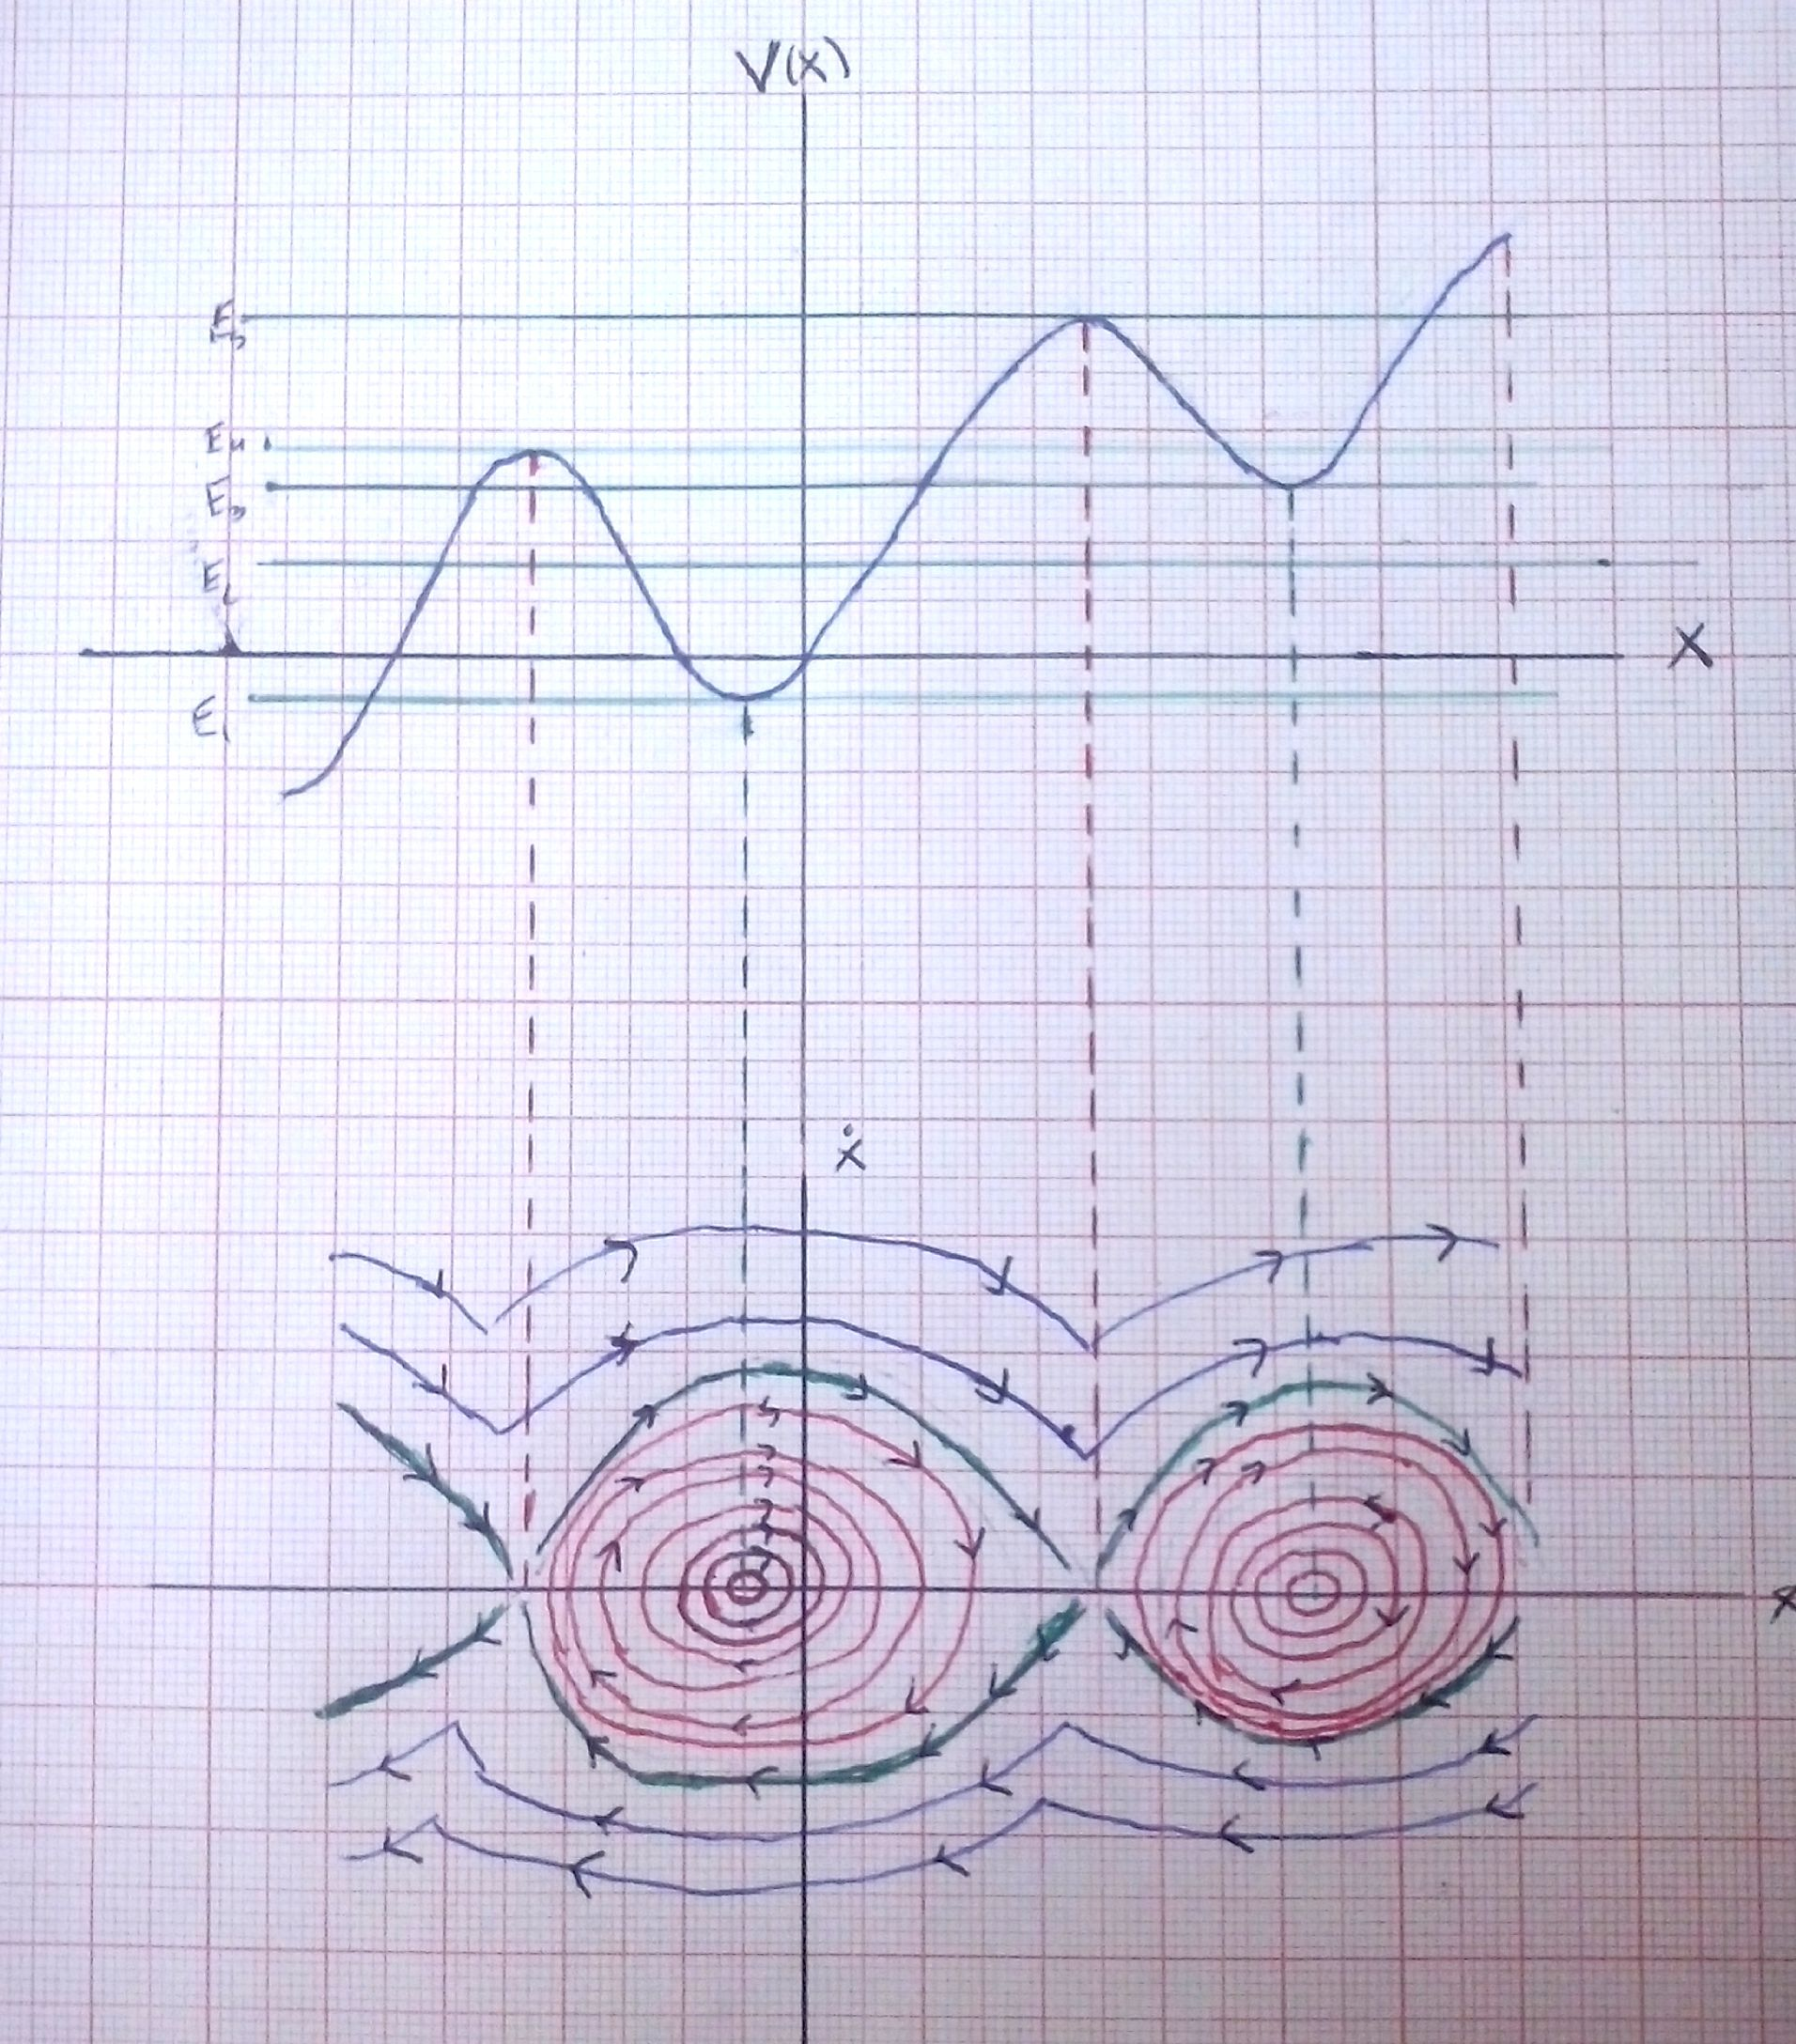
\includegraphics[scale=0.2]{problema1fig2}
 \caption{Problema 1. Diagrama de fases resultante}
 \label{fig:diagramaFase}
\end{figure}


\section{Problema 2}

Demuestre que una trayectoria de Lissajous en el espacio físico de dos 
dimensiones cubre densamente la región a la que tiene acceso si, y sólo si,
las dos frecuencias son inconmensurables.

\vspace{.3cm}

\underline{Solución:} \vspace{.3cm}

Para demostrar este enunciado utilizaremos algunas técnicas de \cite{arnold}, conjunto
con algunas particularidades que desarrollaremos aquí. Comenzaremos con unas definiciones 
importantes las cuales nos permitirán luego demostrar un teorema y un lema que completará
la demostración del enunciado. El problema debe tratarse en el espacio físico, pero 
algunas demostraciones se harán en el espacio de fase, pero su extensión es 
posible.

\vspace{.3cm}

\definicion Dos números $\omega_1$ y $\omega_2$ se llaman racionalmente independientes si la 
relación $k_1\omega_1 + k_2\omega_2 = 0$, con $k_1$ y $k_2$ enteros, que implica que 
$k_1 = k_2 = 0$.

\vspace{.3cm}

Por ejemplo $\sqrt{2}$ y $\sqrt{8}$ son racionalmente dependientes, mientras que 
$\sqrt{6}$ y $\sqrt{8}$ son racionalmente independientes. Podemos ver esta definición
desde otra perspectiva, que está un poco más cercana a la notación en mecánica clásica,

\vspace{.3cm}

\definicion Si la división entre $\omega_1$ y $\omega_2$ es un número 
racional $k_2/k_1$, donde $k_1$ y $k_2$ son enteros, entonces se dice que $\omega_1$ y
$\omega_2$ son \emph{conmensurables}. De lo contrario se llaman \emph{inconmensurables}

\vspace{.3cm}

Para demostrar el enunciado utilizaremos un teorema y un lema definidos sobre un 
toro $T^2$, esto lo hacemos debido a que como es sabido un sistema de dos dimensiones 
como el que tratamos, el espacio de fase es de cuatro dimensiones, pero el espacio $\mathbb{R}^4$
puede descomponerse en la suma directa de dos planos invariantes 

\begin{equation}
 \mathbb{R}^4 = \mathbb{R}_{1,2} + \mathbb{R}_{3,4}.
\end{equation}

En cada uno de estos planos las curvas de fase son círculos $S^1$, para el caso que tratamos, entonces cada 
curva de fase pertenece al producto directo de las curvas de fase en $\mathbb{R}_{1,2}$ y
$\mathbb{R}_{3,4}$, si ambos son círculos entonces obtenemos 


\begin{equation}
 T^2 = S^1 \times S^1,
\end{equation}

llamado un toro dos-dimensional. 

\vspace{.3cm}

\definicion Un conjunto $A$ es denso en todas partes en un espacio $B$ 
si hay un punto del conjunto $A$ en cada vecindad arbitrariamente pequeña de 
cualquier punto del espacio $B$.

\vspace{.3cm}

Podemos entonces enunciar el siguiente teorema,

\vspace{.3cm}

\teorema Si $\omega_1$ y $\omega_2$ son racionalmente dependientes, entonces 
cada curva de fase en el toro $T^2$ es cerrada. Si $\omega_1$ y $\omega_2$ son racionalmente
independientes, entonces las curvas de fase cubren densamente el toro $T^2$. 

\vspace{.3cm}

Para demostrar el teorema primero demostraremos el siguiente lema,

\vspace{.3cm}

\lema Considere una rotación del círculo $S^1$ por un ángulo $\alpha$ que 
es inconmensurable con $2\pi$. Entonces las imágenes de cualquier punto en el círculo 
bajo las rotaciones repetidas

\begin{equation}
 \phi, \phi + \alpha, \phi + 2\alpha, \phi + 3\alpha, \dots (\text{mod} 2\pi),
\end{equation}

forman un conjunto que es denso en todas partes del circulo.

\vspace{.3cm}

\prueba La prueba puede ser deducida de la estructura de los subgrupos cerrados 
de la línea. Comenzamos enunciando el llamado ``principio del hoyo de pájaro'': Si $k+1$ 
objetos yacen en $k$ cajas, entonces al menos uno de las cajas tiene más de un 
objeto. Dividimos el círculo en $k$ intervalos semiabiertos de longitud $2\pi/k$. 
Pero por el principio que enunciamos, entre los primeros $k+1$ puntos de nuestra 
secuencia hay dos que yacen en el mismo intervalo semiabierto. Sean estos puntos 
$\phi+p\alpha$ y $\phi+q\alpha$ con $p>q$. Consideremos $s=p-q$. El ángulo de 
rotación $s\alpha$ difiere de un múltiplo de $2\pi$ por menos de $2\pi/k$. En la secuencia 
de puntos $\phi,\phi+s\alpha,\phi+2s\alpha,\phi+3s\alpha,\dots$ (mod $2\pi$)\footnote{Ver figura 
\mref{fig:problema2fig1}} cada par de puntos adyacentes están a la misma distancia, menor que $2\pi/k$, de cada uno de 
ellos. Sea un numero $\epsilon>0$ dado. Escogiendo $k$, lo suficientemente grande,
podemos tener obtener $2\pi/k < \epsilon$. En cualquier vecindad de $\epsilon$, de 
cualquier punto de $S^1$ hay puntos de la secuencia $\phi+Ns\alpha$. Lo cual prueba
el lema.

\vspace{.2cm} $\hspace{12cm} \square$

\begin{figure}[H]
 \center
 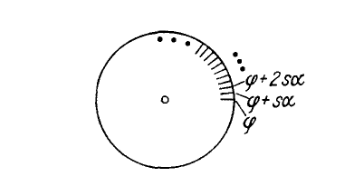
\includegraphics[scale=0.6]{problema2fig1}
 \caption{Los puntos $\phi+Ns\alpha$}
 \label{fig:problema2fig1}
\end{figure}


El lema no utiliza directamente la inconmensurabilidad de $\alpha$ con $2\pi$, pero 
es claro que el lema no es cierto para un $\alpha$ conmensurable con $2\pi$.

\vspace{.3cm}

Estamos en posición entonces para probar el teorema. Aunque todo sea muy matemático 
hasta ahora luego cuando hablemos del caso particular del problema al que nos enfrentamos,
haremos una breve descripción física de la situación.

\vspace{.3cm}

\textbf{Prueba del teorema}: Las trayectorias de fase del flujo que consideramos\footnote{Estamos considerando
un flujo muy similar al que nos encontraremos en el caso del oscilador armónico en 2D.}
sobre la superficie de $T^2$ satisfacen la ecuación diferencial,

\begin{equation}
 \dot{\phi}_1 = \omega_1, \quad \dot{\phi}_2 = \omega_2.
\end{equation}

Las soluciones de esta ecuación tienen la forma

\begin{equation}
 \phi_1 (t) = \phi_1 (0) + \omega_1 t, \quad \phi_2 (t) = \phi_2 (0) + \omega_2 t.
\end{equation}

Sean $\omega_1$ y $\omega_2$ racionalmente dependientes: $k_1\omega_1 + k_2 \omega_2 = 0$,
$k_1^2+k_2^2 \ne 0$. Las ecuaciones en una variable $T$ 

\begin{equation}
 \omega_1 T = 2 \pi k_2, \quad \omega_2 T = - 2 \pi k_1,
\end{equation}

son consistentes. Una solución $T$ de estas ecuaciones es un período de la curva 
cerrada de fase.

\vspace{.3cm}

Sea $\omega_1$ y $\omega_2$ racionalmente independientes. Como dijimos en una definición 
anterior, $\omega_1/\omega_2$ es un número irracional. Consideremos los puntos de 
intersección consecutivos de la curva de fase con el meridiano $\phi_1=0$ (mod $2\pi$). 
Las latitudes de estos puntos son

\begin{equation}
 \phi_{2,k} ) \phi_{2,0} + 2\pi \frac{\omega_2}{\omega_1}k \quad (\text{mod} 2\pi).
\end{equation}

Por el lema, el conjunto de puntos de la intersección es denso en todas partes del 
meridiano. Entonces, las líneas dibujadas desde los puntos de un conjunto que es 
denso en todas partes, en una línea que yace en el plano en una dirección con 
esa línea, forman un subconjunto denso en todas partes del plano. Por lo que la imagen

\begin{equation}
 \tilde{\phi_1}(t) = \phi_1 (t) - 2\pi \left[\frac{\phi_1(t)}{2\pi} \right], \quad
  \tilde{\phi_2}(t) = \phi_2 (t) - 2\pi \left[\frac{\phi_2(t)}{2\pi} \right],
\end{equation}

de la curva de fase en el cuadrado $0 \leq \tilde{\phi_1} < 2\pi $, 
$0 \leq \tilde{\phi_2} < 2\pi $, es densa en todas partes. Por lo que 
una curva de fase de la ecuación que consideramos es densa en todas 
partes del toro.

\vspace{.2cm} \hspace{12cm} $\square$

Consideremos ahora que ya hemos probado el lema y teorema que nos interesaban,
el caso de un oscilador armónico en dos dimensiones. Las componentes de 
la ecuación de movimiento son

\begin{equation}
 \frac{d^2x}{dt^2} + \omega_1^2 x = 0, \qquad \frac{d^2y}{dt^2} + \omega_2^2 x = 0,
\end{equation}

donde $\omega_i = \sqrt{k_i/m}$. La soluciones generales son

\begin{equation}
 x(t) = A_1 \cos{\omega_1 t + \delta_1}, \qquad y(t) = A_2 \cos{\omega_2 t + \delta_2},
\label{eq:solOsci2D}
\end{equation}

donde las constantes $A_i$ y $\phi_i$ dependen de las condiciones iniciales 
$r_0$ y $v_0$. Como vimos anteriormente la naturaleza de la trayectoria descrita 
por \mref{eq:solOsci2D} dependen crucialmente de la proporción de las frecuencias 
angulares $\omega_1/\omega_2$. Démosle un sentido físico aplicado al problema, a las 
ecuaciones que se encuentran dentro de la prueba del teorema. Veíamos que 
si $\omega_1$ y $\omega_2$ eran conmensurables las trayectorias eran cerradas. Esto
significa en el caso del oscilador armónico 2D que cuando la partícula 
ha hecho $k_1$ oscilaciones completas en la dirección $x$, también
habrá hecho $k_2$ oscilaciones completas en la dirección de $y$, y por 
lo tanto ha vuelto a su punto de inicio $r_0$ con la misma velocidad inicial 
$v_0$. El movimiento es periódico en este caso, lo cual lo podemos entender ahora
desde una perspectiva física y matemática.

\vspace{.3cm}

Si $\omega_1$ y $\omega_2$ son inconmensurables, es decir que su proporción 
es un número irracional, habíamos dicho que las trayectorias eran densas 
en todas partes, esto desde la perspectiva del problema que tratamos quiere decir 
que la partícula nunca vuelve a tener sus condiciones iniciales $r_0$ y $v_0$,
entonces nunca pasa dos veces por el mismo punto con la misma velocidad, lo 
que hace claramente q la órbita sea abierta.

\vspace{.3cm}

En el caso del oscilador armónico en 2D las trayectorias del espacio físico
serán figuras de Lissajous cerradas, y periódicas si las frecuencias angulares
son conmensurables, o cubrirán densamente el espacio físicos con figuras
tipo Lissajous describiendo trayectorias abiertas.

\section{Problema 3}

Encuentre la sección de dispersión para un potencial coulombiano repulsivo.

\vspace{.3cm}

\underline{Solución:} \vspace{.3cm}

Antes de dar la solución al problema hay que hacer algunas definiciones importantes, y
encontrar algunas relaciones de la dispersión clásica generalizada que facilitarán
la solución del caso que consideramos. Para esto utilizaremos un conjunto de 
acercamientos al problema desde los libros de mecánica clásica como
\cite{marion, goldstein}.

\vspace{.3cm}

Consideremos la situación mostrada en la figura \mref{fig:problema3fig1}

\begin{figure}[H]
 \center
 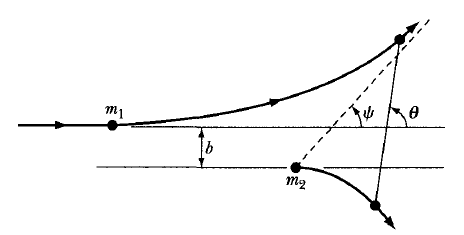
\includegraphics[scale=0.5]{problema3fig1}
 \caption{Representación esquemática del problema de dispersión visto desde 
 el sistema de laboratorio.}
 \label{fig:problema3fig1}
\end{figure}

que ilustra una colisión en el sistema de coordenadas del laboratorio\footnote{Comúnmente 
suele llamarse sistema de coordenadas de laboratorio a uno que está en reposo
viendo el sistema ocurrir, como un científico viendo el fenómeno parado 
o sentado (si es muy largo) ocurrir.} cuando una fuerza repulsiva existe 
entre $m_1$ y $m_2$. 

\vspace{.3cm}

\definicion Llamaremos parámetro de impacto, $b$, a la distancia 
más cercana a la que la partícula $m_1$ se acercaría a la vecindad de $m_2$
si hubiera fuerza actuando sobre las partículas.

\vspace{.3cm}

En la mayoría de los casos, no podemos escoger ni medir directamente $b$,
por lo tanto, debemos reducirnos a hablar, en estas situaciones, de la probabilidad
para varios ángulos de dispersión $\theta$.

\vspace{.3cm}

Consideramos ahora la distribución de ángulos de dispersión que resultan 
de la colisión con varios parámetros de impacto. Para hacer esto, asumamos
que tenemos un haz estrecho de partículas, cada una con masa $m_1$ y energía 
$T_0$. Dirigimos este haz hacia una pequeña región del espacio que contiene 
una colección de partículas, cada una con una masa $m_2$ en reposo. 

\vspace{.3cm}

\definicion La intensidad o flujo de intensidad $I$ de las partículas
incidentes, es el número de partículas pasando por unidad de tiempo a través 
de una unidad de área normal a la dirección del haz. 

\vspace{.3cm}

Si asumimos que la fuerza entre $m_1$ y $m_2$ decae con la distancia 
lo suficientemente rápido, entonces luego del encuentro, el movimiento 
de la partícula dispersada asintóticamente se acerca a una línea 
recta con un ángulo bien definido $\theta$ entre las dirección inicial
del movimiento y la final.

\vspace{.3cm}

\definicion La sección de dispersión diferencial $\sigma (\theta)$ en el 
sistema de Centro de Masa (CM) del sistema para la dispersión dentro de 
un elemento de ángulo sólido $d\Omega'$ a un ángulo particular $\theta$ CM,
es:

\begin{equation}
 \sigma(\theta) = \frac{\left(\text{\parbox{20em}{número de interacciones por partículas objetivo que
 llevan a una dispersión dentro de d$\Omega'$ a un ángulo $\theta$}} \right)}{\text{Número de 
 partículas incidentes por unidad de área}}.
 \label{eq:disper1}
\end{equation}

Si $dN$ es el número de partículas dispersadas dentro de $d\Omega'$ por unidad
de tiempo, entonces la probabilidad de dispersión dentro de $d\Omega'$ de 
un haz incidente es

\begin{equation}
 \sigma (\theta) d\Omega' = \frac{dN}{I}.
 \label{eq:disper2}
\end{equation}

Podemos escribir también,

\begin{equation}
 \sigma(\theta) = \frac{d\sigma}{d\Omega'} = \frac{1}{I}\frac{dN}{d\Omega'}.
 \label{eq:disper3}
\end{equation}

El hecho de que $\sigma(\theta)$ tenga las dimensiones de área por estereorradián\footnote{El estereorradián 
se define haciendo referencia a una esfera de radio $r$. Si el área de una porción de esta esfera es $r^2$, un estereorradián es el ángulo sólido comprendido entre esta porción y el centro de la esfera.}
da lugar al término \emph{sección de dispersión}. El hecho de que asumimos que 
la fuerza entre las partículas es central, la dispersión tiene simetría
axial, podemos entonces hacer la integración sobre el ángulo azimutal 
para obtener $2\pi$, y luego el elemento de ángulo sólido $d\Omega'$ está
dado por 

\begin{equation}
 d\Omega' = 2\pi \sen{\theta} d\theta.
 \label{eq:disper4}
\end{equation}

Si consideramos, por un momento, la dispersión de una partícula de 
masas $\mu$ por un centro de fuerza, entonces la figura \mref{fig:problema3fig2},
muestra que el número de partículas con parámetros de impacto dentro de 
un rango $db$ a una distancia $b$ deben corresponder con el número de 
partículas dispersadas dentro del rango angular $d\theta$ a una ángulo $\theta$,
entonces

\begin{equation}
 I2\pi b db = - I \sigma(\theta)2\pi\sen{\theta}d\theta,
 \label{eq:disper5}
\end{equation}

donde $db/d\theta$ es negativo, debido a que hemos asumidos que la fuerza 
es tal que la cantidad de deflexión angular decrece monótonamente aumentando 
de parámetro de impacto. 

\begin{figure}[H]
 \center
 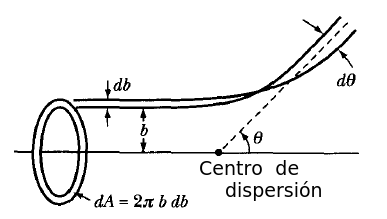
\includegraphics[scale=0.5]{problema3fig2}
 \caption{Problema equivalente de un cuerpo de masa $\mu$ dispersado 
 por un centro de fuerzas}
 \label{fig:problema3fig2}
\end{figure}

Entonces,

\begin{equation}
 \sigma(\theta) = \frac{b}{\sen{\theta}}\left\| \frac{db}{d\theta} \right\|.
 \label{eq:disper6}
\end{equation}

Podemos obtener ahora una relación entre el parámetro de impacto $b$ y el 
ángulo de dispersión usando la figura \mref{fig:problema3fig3}.

\begin{figure}[H]
 \center
 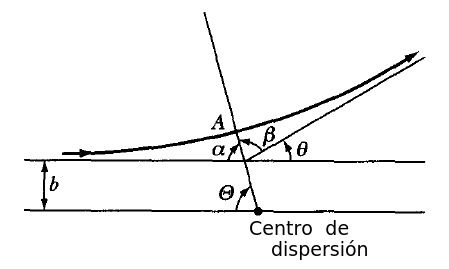
\includegraphics[scale=0.5]{problema3fig3}
 \caption{Geometría de una partícula dispersada en un campo central. El punto
 A es la distancia de mayor acercamiento.}
 \label{fig:problema3fig3}
\end{figure}

Como puede demostrarse de manera sencilla, el cambio de ángulo 
de una partícula de masa $\mu$ moviéndose en un campo central está
dado por ($l$ es la velocidad angular y $V$ la energía potencial)

\begin{equation}
 \Delta \Theta = \int_{r_{min}}^{r_{max}} \frac{(l/r^2)dr}{\sqrt{2\mu[
 E - V - (l^2/2\mu r^2)}}.
 \label{eq:disper7}
\end{equation}

Entonces el movimiento de una partícula en un campo central es simétrico
respecto al punto de mayor acercamiento al centro de fuerza ($A$), lo que
hace que los ángulos $\alpha$ y $\beta$ sean iguales. Tenemos entonces que 

\begin{equation}
 \theta = \pi - 2\Theta.
 \label{eq:disper8}
\end{equation}

Para el caso en que $r_{max} = \infty$, el ángulo $\Theta$ está dado por

\begin{equation}
 \Delta \Theta = \int_{r_{min}}^{\infty} \frac{(b/r^2)dr}{\sqrt{1 -
 (b^2/r^2) - (U/T_0')}}.
 \label{eq:disper9}
\end{equation}

Donde hemos usado el hecho de que $l=b\sqrt{2\mu T_0'}$, y hemos puesto 
$E = T_0'$, debido a que la energía total $E$ debe ser igual a la energía
cinética $T_0'=\frac{1}{2} \mu u_1^2$ en $r=\inf$ donde $V=0$.

\vspace{.3cm}

Estamos ahora en posición para calcular lo solicitado en el problema, nos piden
que consideremos un potencial coulombiano repulsivo, por lo tanto podemos 
escribir este como

\begin{equation}
 V(r) = \frac{k}{r}.
 \label{eq:coulombPot}
\end{equation}

Entonces la ecuación \mref{eq:disper9}, se convierte en

\begin{equation}
 \Theta = \int_{r_{min}}^{\infty} \frac{(b/r)dr}{\sqrt{r^2-(k/T_0')r-b^2}},
\end{equation}

que al integrarse resulta (haciendo cambio de variable $b/r$ y de ahí un
proceso un poco largo) en

\begin{equation}
 \cos{\Theta} = \frac{(\kappa/b)}{\sqrt{1+(\kappa/b)^2}},
 \label{eq:CosThet}
\end{equation}

donde hemos definido

\begin{equation}
 \kappa = \frac{k}{2T_0'}.
\end{equation}

Podemos reescribir \mref{eq:CosThet} como

\begin{equation}
 b^2=\kappa^2 \tan^2{\Theta}.
\end{equation}

Pero de la ecuación \mref{eq:disper8}, $\Theta = \pi /2 - \theta/2$,
entonces

\begin{equation}
 b = \kappa \cot{\theta/2}.
\end{equation}

Entonces

\begin{equation}
\frac{db}{d\theta} = - \frac{\kappa}{2} \frac{1}{\sin^2{\theta/2}}.
\end{equation}

Y de la ecuación \mref{eq:disper6} tenemos que 

\begin{equation}
 \sigma (\theta) = \frac{\kappa^2}{2}\frac{\cot{\theta/2}}{\sen{\theta}\sen^2{\theta/2}}.
\end{equation}

Pero,

\begin{equation}
 \sen{\theta} = 2\sen{\theta/2}\cos{\theta/2}.
\end{equation}

Por lo que,

\begin{equation}
  \sigma (\theta) = \frac{\kappa^2}{4}\frac{1}{\sen^4{\theta/2}},
\end{equation}

o,

\begin{equation}
 \boxed{\sigma (\theta) = \frac{k^2}{(4T_0')^2}\frac{1}{\sen^4{\theta/2}}.}
\end{equation}

Que es la conocida sección de dispersión para un potencial coulombiano repulsivo,
obtenida por primera vez por Rutherford, en 1911, en su estudio de la dispersión de 
partículas $\alpha$ por un núcleo atómico, curiosamente, este fue uno o el más famoso
trabajo de Rutherford y lo hizo luego de ya haber ganado el premio nobel en 1908.

\section{Problema 4}

Demuestre que una partícula moviéndose en una dimensión y sujeta a la 
acción de una fuerza 

$$ 
f = -kx^{2n+1} \qquad n \quad \text{entero positivo,}
$$

oscilará con un período proporcional a $A^{-n}$, donde $A$ es la amplitud 
de la oscilación. ¿Es esto válido cuando $n<0$?

\vspace{.3cm}

\underline{Solución:} \vspace{.3cm}

Debido a la forma de la fuerza que nos dan en el problema, y al hecho de que en una 
dimensión todas las fuerzas que dependen solo de $x$ son conservativas, entonces 
podemos escribir \cite{saletan},

\begin{equation}
 F(x) = - \frac{dV(x)}{dx}.
 \label{eq:potencial1}
\end{equation}

Por otra parte la energía total del sistema puede escribirse como,

\begin{equation}
 E = \frac{1}{2} m\dot{x}^2 + V(x).
 \label{eq:energTotal1}
\end{equation}

La ecuación \mref{eq:energTotal1} puede resolverse para $1/\dot{x}=dt/dx$, lo que 
resulta en 

\begin{equation}
 \int_{t_0}^t dt = \sqrt{\frac{m}{2}} \int_{x_0}^{}x \frac{dx}{\sqrt{E - V(x)}}.
\end{equation}

Que resulta en 

\begin{equation}
  t - t_0 = \sqrt{\frac{m}{2}} \int_{x_0}^{}x \frac{dx}{\sqrt{E - V(x)}},
\end{equation}

donde $x_0$ es la posición de la partícula en el tiempo $t_0$, y $x$ es la posición 
en el tiempo $t$. Si en una gráfica de $V(x)$ sobre $x$, podemos encontrar una 
región en la cual una partícula, con una energía dada, se encuentre constreñida 
a moverse alrededor de un mínimo, decimos que la misma oscila, o que el movimiento 
es periódico sobre esa región, en el cual puede demostrarse con facilidad que 
los límites de la oscilación serán entre el valor $-A$ y $A$, donde $A$ es la amplitud 
de la oscilación.

\vspace{.3cm}

\definicion El período de una oscilación es el tiempo que le toma a una partícula 
ir de $-A$ a $A$ y volver de nuevo, donde $A$ es la amplitud de la oscilación.

\vspace{.3cm}

Debido a esta definición, y al hecho de que el tiempo que le toma a la partícula ir 
de $-A$ a $A$ es el mismo que le toma para ir de $A$ a $-A$ (si el potencial 
es simétrico), podemos escribir el período como

\begin{equation}
 T = 2 \sqrt{m/2} \int_{-A}^A \frac{dx}{\sqrt{E - V(x)}} = \sqrt{2m} \int_{-A}^A \frac{dx}{\sqrt{E - V(x)}}.
\label{eq:periodo1}
\end{equation}


Con los resultados obtenidos podemos ahora dar solución al problema. En el 
enunciado nos dicen que la partícula está sujeta a una fuerza $F(x) = - kx^{2n+1}$,
por lo que 

\begin{gather}
 \int_{0}^{V(x)} dV(x) = k \int_0^x x^{2n+1} dx, \\
 \therefore V(x) = \Theta x^{2(n+1)},
 \label{eq:potencial2}
\end{gather}

donde hemos definido $\Theta = k/2(n+1)$. Por otra parte, en la oscilación de una partícula
los momentos iniciales y finales de la oscilación son aquellos en los que la velocidad es 
igual a cero, o dicho de otra manera en los que la energía total es igual al potencial,
entonces

\begin{equation}
 E = V(A) =  \Theta A^{2(n+1)}.
 \label{eq:energTotal2}
\end{equation}

Introduciendo los resultados de \mref{eq:potencial2} y \mref{eq:energTotal2} en 
\mref{eq:periodo1} obtenemos

\begin{equation}
 T = \sqrt{2m} \int_{-A}^A \frac{dx}{\sqrt{\Theta A^{2(n+1)} - \Theta x^{2(n+1)}}} = 
 \sqrt{2m} \int_{-A}^A \frac{dx}{\sqrt{\Theta} \sqrt{A^{2(n+1)} - x^{2(n+1)}}}.
 \label{eq:periodo2}
\end{equation}

Si hacemos el cambio de variables $x = A \xi$, entonces 

\begin{equation}
 dx = A d\xi,
\end{equation}

y los límites de integración cambian a 

\begin{align*}
%
 (\text{inferior}) \quad x &= - A \Rightarrow \xi = A / -A = -1, \\
 %
 (\text{superior}) \quad x &= A \Rightarrow \xi = A / A = 1,
 %
\end{align*}

entonces \mref{eq:periodo2} se transforma en 

\begin{align}
 \begin{split}
  %
  T &= \sqrt{\frac{2m}{\Theta}} \int_{-1}^1 \frac{A d\xi}{\sqrt{A^{2(n+1)} - (A\xi)^{2(n+1)}}}, \\
  %
    &= \sqrt{\frac{2m}{\Theta}} \int_{-1}^1 \frac{Ad\xi}{A^{2(n+1)}[1 - \xi^{2(n+1)}]}, \\
  %
    &= \sqrt{\frac{2m}{\Theta}} \int_{-1}^1 \frac{Ad\xi}{A^{(n+1)}\sqrt{1-\xi^{2(n+1)}}}.
  %
 \end{split}
\end{align}

Y debido a que $A/A^{(n+1)} = A^{-n}$, tenemos que 

\begin{equation}
 \boxed{T = \sqrt{\frac{2m}{\Theta}} A^{-n} \int_{-1}^1 \frac{d\xi}{\sqrt{1-\xi^{2(n+1)}}}.}
\end{equation}

Y debido a que la integral es una constante, entonces hemos demostrado que $T \propto A^{-n}$.

\vspace{.3cm}

Debido a la forma del potencial, si $n=0$,

\begin{equation}
 F(x) = -k x.
\end{equation}

Que es simplemente el caso del oscilador armónico de una dimensión. Por otra parte si 
$n$ es negativo, digamos que $n=-1$, entonces 

\begin{equation}
 F = - k x^{-1} \Rightarrow V(x) = k \ln{|x/c|},
\end{equation}

donde hemos puesto $\ln{|c|}$ como constante de integración. Este tipo de potenciales
no puede generar oscilaciones periódicas debido a que no tiene mínimos, y aparte 
es una función discontinua debido a que no contiene al 0 en su dominio. Por lo que 
esta solución no funciona para un $n$ negativo ya que daríamos la errónea conclusión de
que por ejemplo si $n=-1$ entonces el período sería proporcional a $A$, lo cual se 
puede demostrar siguiendo un procedimiento similar al que llevamos a cabo en la solución 
del problema. Pero por la descripción del potencial que acabamos de hacer vemos que 
sería un error conjeturar tal cosa, por lo cual esta solución no es válida cuando 
$n<0$.

\section{Problema 5}

Grafique las proyecciones $(\theta,r)$, $(\theta,\dot{r})$, $(r,\dot{r})$,
y $(r,\dot{\theta})$ en el espacio de fase $(\theta,r,\dot{\theta},\dot{r})$
(ojo no se trata dela órbita) de una partícula sujeta a una fuerza central 
gravitacional. Considere tanto casos con energía total positiva, como 
negativa.

\vspace{.3cm}

\underline{Solución:} \vspace{.3cm}

Consideramos el espacio de fases de una partícula sujeta a una fuerza gravitacional;
este espacio de fases de 4-dimensional, y debido a la dificultad de conseguir un 
programa que haga gráficos en 4 dimensiones (serían bien caros), y a la dificultad 
que tenemos para hacerlo en un cuaderno al ser seres tridimensionales, lo máximo que 
podemos hacer es dibujar las proyecciones de este espacio de fase en los planos que
la forman, en este caso $(\theta,r)$ $(\theta,\dot{r})$, $(r,\dot{r})$ y $(r,\dot{\theta})$\footnote{
Es claro que es equivalente graficar la proyección de $(a,b)$ a la de $(b,a)$}.

\vspace{.3cm}

Todos los códigos con los que realicé estas gráficas son libres y se encuentran en 
el un NoteBook de Python, en \href{https://github.com/FavioVazquez/MecanicaClasica-PCF/blob/master/Tarea3/Problema5.ipynb}{\color{blue}.:este link:..}.
Fueron hechos com Matplotlib\footnote{\href{http://matplotlib.org/}{http://matplotlib.org/}} usando
la función \texttt{plot.polar()} algunos, otros con \texttt{plot.plot()} y el último 
con \texttt{plot.streamplot()}.

\vspace{.3cm}

Comencemos por $(r,\theta)$. En este caso tenemos la  ecuación para las órbitas que es

\begin{equation}
 r = \frac{\alpha}{1 + \epsilon \cos{\theta}},
 \label{eq:rtita}
\end{equation}

donde,

\begin{align}
 \begin{split}
  %
  \alpha &= \frac{l^2}{m k}, \\
  %
  \epsilon &= \sqrt{1 + \frac{2El^2}{mk^2}},
 \end{split}
\end{align}

A $\epsilon$ se le conoce como la excentricidad, y a $2\alpha$ como el latus rectum 
de la órbita. Esta ecuación \mref{eq:rtita} es la de una cónica con uno de sus focos 
en el origen. Y tenemos los siguientes casos\footnote{Los valores de $E$ menores que 
$V_{min}= -(mk^2/2l^2)$ no producen movimiento físico real, debido que para esos 
casos $\dot{r}^2 < 0$ y la velocidad es imaginaria (y aunque lo intentemos mucho
no podremos imaginarla)}:

\begin{itemize}
 \item $\epsilon > 1, \qquad E>0$ $\Rightarrow$ Hipérbola

\begin{figure}[H]
 \center 
 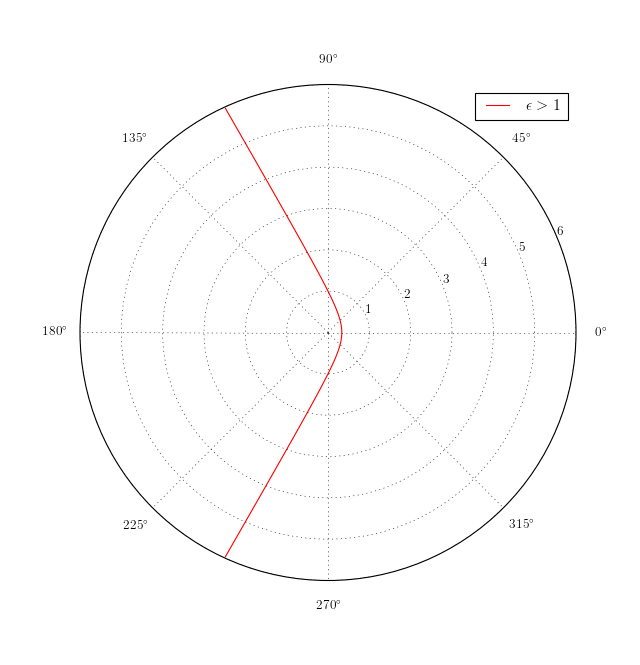
\includegraphics[scale=0.5]{problema5fig1}
 \caption{Caso $\epsilon > 1$}
 \label{fig:hiperbola}
\end{figure}

\newpage %Ojo con este newpage puede cambiar

 \item $\epsilon = 1, \qquad E=0$ $\Rightarrow$ Parábola


\begin{figure}[H]
 \center 
 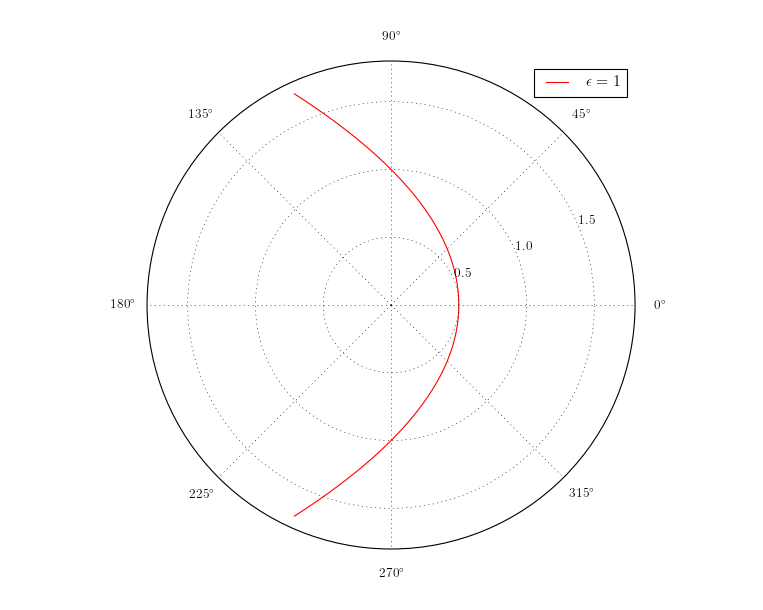
\includegraphics[scale=0.45]{problema5fig2}
 \caption{Caso $\epsilon = 1$}
 \label{fig:parabola}
\end{figure}

 \item $\epsilon = 0, \qquad E=V_{min}$ $\Rightarrow$ Círculo

\begin{figure}[H]
 \center 
 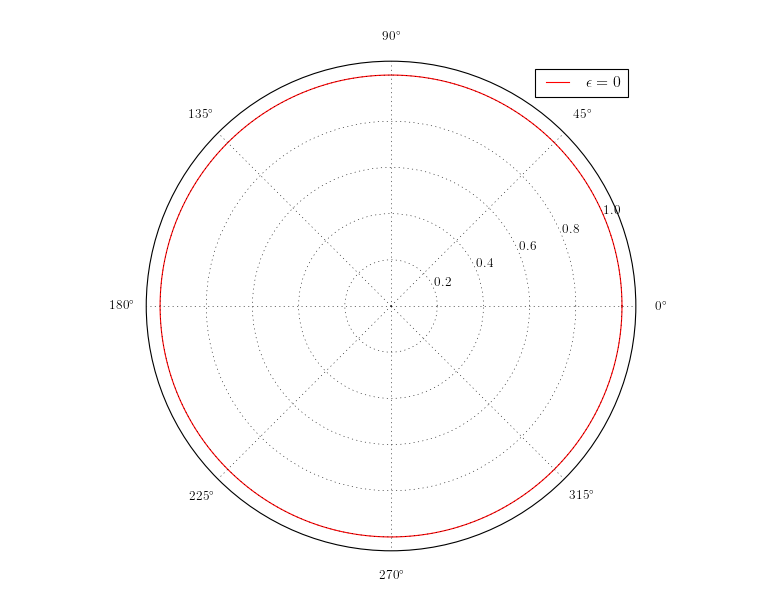
\includegraphics[scale=0.4]{problema5fig3}
 \caption{Caso $\epsilon = 0$}
 \label{fig:circulo}
\end{figure}

\newpage

 \item $0 < \epsilon < 1, \qquad  0 < E < V_{min}$ $\Rightarrow$ Elipse

\begin{figure}[H]
 \center 
 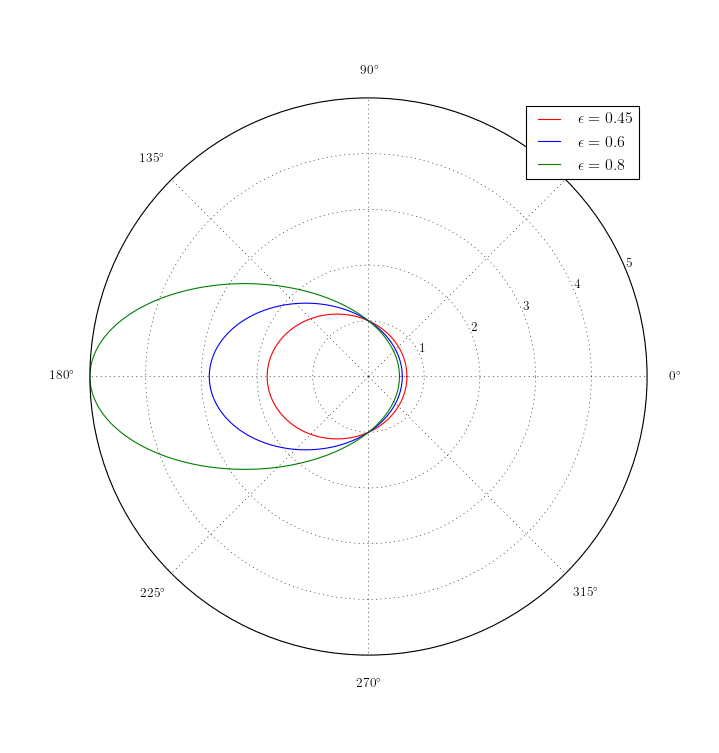
\includegraphics[scale=0.45]{problema5fig4}
 \caption{Caso $0 < \epsilon < 1$}
 \label{fig:elipse}
\end{figure}

\end{itemize}

Para $(\dot{\theta},r)$, podemos utilizar el impulso angular, que se expresa como

\begin{equation}
 l = mr^2\dot{\theta},
\end{equation}

que si despejamos $\dot{\theta}$, tendremos a $\dot{\theta}$ en función de $r$,

\begin{equation}
 \dot{\theta} = \frac{l}{mr^2}.
\end{equation}

Una función sencilla, positiva definida de la siguiente forma de la figura \mref{fig:titaDotR},
vemos que $\dot{\theta}$ decrece de forma cuadrática con $r$ lo cual es lo esperado.

\begin{figure}[H]
 \center 
 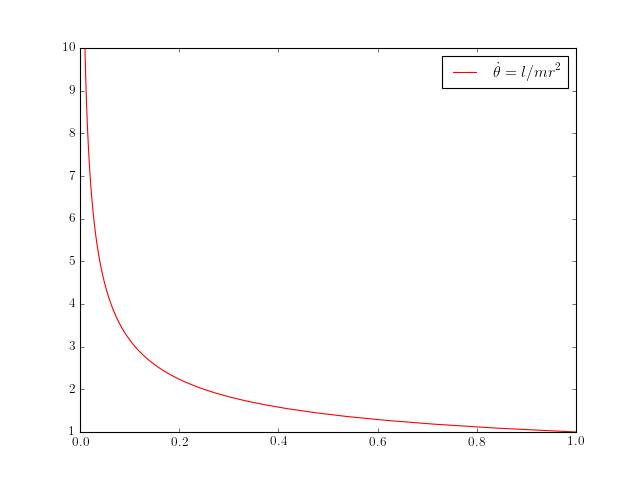
\includegraphics[scale=0.5]{problema5fig5}
 \caption{Gráfico de  $\dot{\theta} = \frac{l}{mr^2}$}
 \label{fig:titaDotR}
\end{figure}

Para el caso de $(\dot{r},\theta)$, podemos utilizar el hecho de que 

\begin{equation}
 \frac{dr}{dt} = \frac{dr}{d\theta}\frac{d\theta}{dt}.
\end{equation}

Derivamos entonces la ecuación \mref{eq:rtita} con respecto a $\theta$ y multiplicamos 
por $\dot{\theta}$, (recordemos que $\dot{\theta} = l/mr^2$ y que $r=\frac{\alpha}{1+\epsilon\cos{\theta}}$)

\begin{align}
 \begin{split}
  %
  \frac{dr}{dt} &= \frac{\cancel{\alpha'(1+\epsilon \cos{\theta})}-\alpha(1+\epsilon 
  \cos{\theta})'}{(1+\epsilon\cos{\theta})^2} \dot{\theta}, \\
  %
		&= \frac{\alpha\epsilon \sen{\theta}}{(1+\epsilon\cos{\theta})^2} 
		\frac{l}{mr^2}, \\
  %
		&= \frac{\cancel{\alpha}\epsilon\sen{\theta}}{\cancel{(1+\epsilon\cos{\theta})^2}}
		\frac{l}{m}\frac{\cancel{(1+\epsilon\cos{\theta})^2}}{\alpha^{\cancel{2}}}.
 \end{split}
\end{align}

\begin{equation}
 \therefore \dot{r}(\theta) = \frac{\alpha l \epsilon \sen{\theta}}{m}.
\end{equation}

Consideremos los siguientes casos

\begin{itemize}
 \item $\epsilon > 1, \qquad E > 0$
 \item $\epsilon = 1, \qquad E = 0$
 \item $ 0 <\epsilon < 1, \qquad V_{min} < E < 0$ 
\end{itemize}

Que son elipses, como las que vemos en la figura \mref{fig:rDotTita}

\begin{figure}[H]
 \center 
 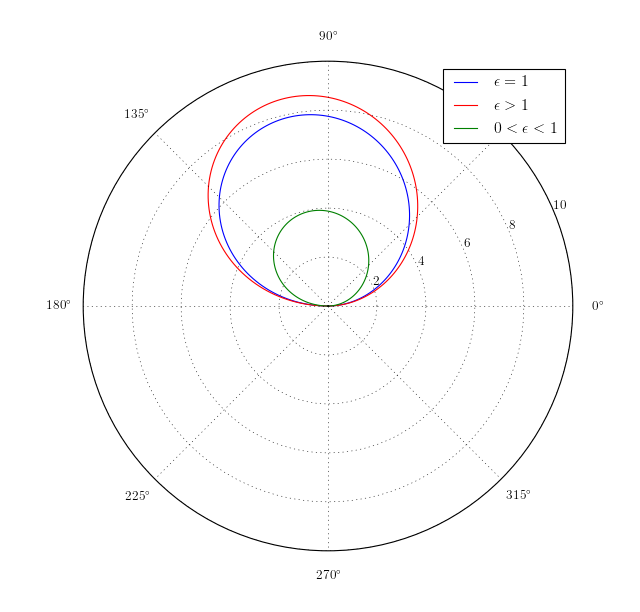
\includegraphics[scale=0.5]{problema5fig6}
 \caption{Gráfico de $\dot{r}(\theta) = \frac{\alpha l \epsilon \sen{\theta}}{m}$ 
 para distintos $\epsilon$}
 \label{fig:rDotTita}
\end{figure}

Para el caso de $(\dot{r},r)$, podemos utilizar la energía total para el caso
de un potencial gravitatorio $V(x) = - k/r$, que tiene la siguiente forma 

\begin{equation}
 E = \frac{1}{2} m\dot{r}^2 + \frac{l^2}{2mr^2} - \frac{k}{r},
\end{equation}

y despejamos $\dot{r}$,

\begin{equation}
 \dot{r} = \pm \sqrt{E - \frac{l^2}{2mr^2} + \frac{k}{r}}.
\end{equation}

El tratamiento que haremos con en este caso será diferente, y lo haremos considerando 
la ecuación diferencial, y el trazaremos el retrato de fase para $(\dot{r},r)$, considerando
el gráfico muy conocido para el potencial efectivo de el problema gravitacional. Parafrasearemos 
el comentario de este gráfico hecho en \cite{saletan} para completar el entendimiento del
problema.

\vspace{.3cm}

En este caso, tomando a $l$ como constante, tendremos el gráfico \mref{fig:rDotR}. Las 
curvas cerradas de este retrato de fase corresponden a estados ligados, en los que 
la partícula tiene una distancia mínima y máxima del centro de fuerza; en el espacio de
configuración esto significa que la partícula está rotando respecto a el centro de 
fuerza. Entonces estos estados ligados forman las órbitas que ya obtuvimos. Estos 
estados tienen todos energías negativas $E$ y las órbitas del espacio de fase de 
velocidad cruzan al eje $r$ en puntos que dependen de $E$. Mientras más grande $E$ (más 
cercano a cero), más cercano será el punto de cruce interno ($r$ mínimo) al origen y más 
lejano el externo ($r$ máximo) del mismo. Las energías negativas terminan en $E=0$, cuando 
el punto de cruce externo se va a $r=\infty$. Esta es la separatriz para este problema, y 
corresponde a una órbita \textbf{parabólica} en el espacio de configuración (ver figura \mref{fig:parabola}).
Mientras más pequeño $E$, mas lejano el punto de cruce interno y más cercano 
el externo, hasta que se encuentran en un punto, que corresponde a un $r$ fijo, 
o a una órbita \textbf{circular} en el espacio de configuración (ver figura \mref{fig:circulo}),
para un valor dado de $l$. Este es el único punto singular de este sistema. Las
órbitas del espacio de fase de velocidad para valores negativos de $E$, entre cero 
y este límite inferior corresponden a \textbf{elipses} en el espacio de configuración (ver 
figura \mref{fig:elipse}). Las órbitas del espacio de fase de velocidad para $E>0$, 
cruzan el eje $r$ solo una vez, entonces cada órbita tiene una asíntota, para $r$ grande,
que es paralela al eje $r$ en el espacio de fases de velocidad. La distancia de 
esta órbita desde el eje $r$ es la velocidad mínima $|\dot{r}|$ a esa energía. Estas 
órbitas en el espacio de configuración para $E>0$ correspondan a órbitas \textbf{hiperbólicas}
(ver figura \mref{fig:hiperbola}.


\begin{figure}[H]
 \center 
 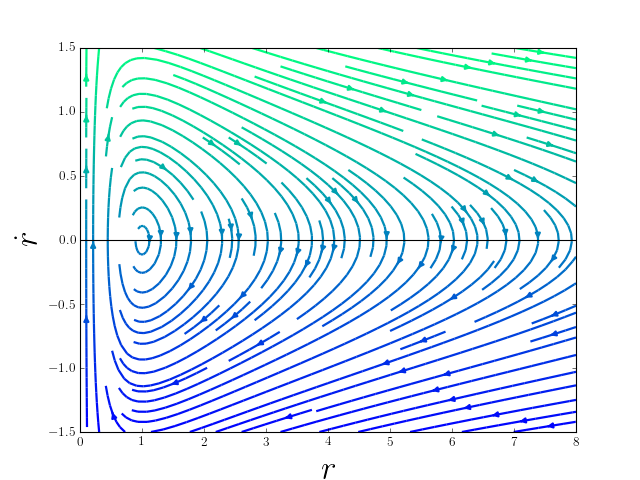
\includegraphics[scale=0.5]{problema5fig7}
 \caption{Gráfico de $(\dot{r},r)$}
 \label{fig:rDotR}
\end{figure}


\begin{thebibliography}{10}
 \bibitem{arnold}
 V.I. Arnold, \emph{Ordinary Differential Equations}, Springer-Verlang,
 3ra edición, 1992.
 \bibitem{marion}
 S. Thronton y J. Marion, \textit{Classical dynamics of particles and systems}, Thomson Brooks/Cole,
 5ta edición, 2004.
 \bibitem{goldstein}
 H. Goldstein, \emph{Classical Mechanics}, Addison-Wesley, 2da edición,
 1980.
 \bibitem{saletan}
 J. José y E. Saletan, \emph{Classical dynamics: A contemporary approach}, Cambridge University Press,
 1998.
\end{thebibliography}

\end{document}
